\ifdefined\pdfminorversion\pdfminorversion=7\fi
\documentclass[aspectratio=169,10pt]{beamer}
% English slides with a separate Chinese speaker script: use pdfLaTeX.
\newif\ifChineseSlides
\ChineseSlidesfalse
\newcommand{\LatinFontPackage}{FiraSans}
\newcommand{\CJKFontSet}{fandol}
\definecolor{SlideBlue}{HTML}{00498A}
\definecolor{SlideBlueDark}{HTML}{1F3A5F}
\definecolor{SlideRed}{HTML}{C8102E}
\definecolor{SlideLight}{HTML}{CCDEEC}
\definecolor{SlideGreen}{HTML}{2E7D32}
\definecolor{SlideGray}{HTML}{595959}
\definecolor{SlideInk}{HTML}{1A1A1A}
\title[Attention Is All You Need]{Attention Is All You Need}
\subtitle{Sequence transduction without recurrence}
\author{Anonymous Authors}
\newcommand{\Presenter}{Presented by Anonymous Presenter}
\institute{}
\newcommand{\HeaderInstitution}{}
\newcommand{\Contact}{}
\newcommand{\TalkType}{10-minute conference oral}
\date{}

\usepackage{paper-slides}
\usepackage{appendixnumberbeamer}
\pdfstringdefDisableCommands{\def\translate#1{#1}}
\hypersetup{pdftitle={Attention Is All You Need -- 10-minute oral},
  pdfauthor={Anonymous Presenter},pdfsubject={Presentation of Vaswani et al., 2017; arXiv v7}}
\newcommand{\source}[1]{\par\smallskip{\footnotesize\color{SlideGray}#1\par}}
% This anonymous deck has no header affiliation; use that space for the title.
\setbeamertemplate{frametitle}{%
  \vskip0.6em
  \begin{minipage}[t]{\textwidth}\raggedright
    {\color{SlideBlue}\bfseries\fontsize{16}{18}\selectfont\insertframetitle\par}
  \end{minipage}\par
  \vskip3pt{\color{SlideBlue}\rule{\textwidth}{1pt}}\par
  \vskip2pt{\small\color{SlideGray}\insertframesubtitle\par}
  \vskip2pt}
\setbeamertemplate{title page}{%
  \begin{center}
    {\small\color{SlideGray}\TalkType\par}\vspace{1em}
    {\color{SlideBlue}\bfseries\fontsize{24}{28}\selectfont\inserttitle\par}
    \vspace{0.55em}{\large\color{SlideBlueDark}\insertsubtitle\par}
    \vspace{0.8em}{\color{SlideRed}\rule{0.42\textwidth}{1.4pt}\par}
    \vspace{0.7em}{\small Paper by Ashish Vaswani, Noam Shazeer, Niki Parmar, Jakob Uszkoreit,\par
      Llion Jones, Aidan N. Gomez, {\L}ukasz Kaiser, and Illia Polosukhin\par}
    \vspace{0.65em}{\small\color{SlideGray}NeurIPS 2017 \enspace $\cdot$ \enspace arXiv:1706.03762v7\par}
    \vspace{0.75em}{\small\color{SlideBlue}\Presenter\par}
  \end{center}}

\begin{document}
% Slide 1 | title | 20 s. Source: ms.tex title/authors/abstract, PDF p. 1.
\begin{frame}[plain,label=title]
  \titlepage
\end{frame}

% Slide 2 | motivation | 45 s. Sources: introduction.tex:3-13;
% why_self_attention.tex, Table 1. Diagrams are supplemental presenter illustrations.
\begin{frame}[label=motivation]{Must sequence modeling be sequential?}
  \takeaway{Self-attention lets positions exchange information directly within a layer.}
  \begin{columns}[t,onlytextwidth]
    \begin{column}{0.47\textwidth}
      \kw{Recurrence: follow the chain}
      \begin{center}
      \begin{tikzpicture}[>=Stealth,x=1.25cm,y=1cm,
        state/.style={draw=SlideBlue,fill=SlideLight!40,minimum size=0.8cm}]
        \path[use as bounding box] (0.55,-0.45) rectangle (4.45,1.0);
        \foreach \i in {1,...,4} {\node[state] (r\i) at (\i,0) {$h_\i$};}
        \foreach \i/\j in {1/2,2/3,3/4} {\draw[->,thick] (r\i)--(r\j);}
      \end{tikzpicture}
      \end{center}
      Each state waits for the previous state.\par\medskip
      Distant signals traverse many steps.
    \end{column}
    \begin{column}{0.47\textwidth}
      \kw{Self-attention: connect positions}
      \begin{center}
      \begin{tikzpicture}[>=Stealth,x=1.25cm,y=1cm,
        state/.style={draw=SlideGreen,fill=SlideGreen!8,minimum size=0.8cm}]
        \path[use as bounding box] (0.55,-0.45) rectangle (4.45,1.0);
        \foreach \i in {1,...,4} {\node[state] (a\i) at (\i,0) {$x_\i$};}
        \foreach \i/\j in {1/2,2/3,3/4} {\draw[<->,thick,SlideGreen] (a\i)--(a\j);}
        \draw[<->,thick,SlideGreen] (a1.north) to[bend left=30] (a4.north);
      \end{tikzpicture}
      \end{center}
      Compute token interactions together.\par\medskip
      Distant positions connect directly.
    \end{column}
  \end{columns}
  \vspace{0.25em}
  \begin{block}{The paper's question}
    Can attention replace recurrence and convolution for machine translation?
  \end{block}
  \source{Vaswani et al., Sections 1 and 4. Illustrations show selected connections, not full architectures.}
\end{frame}

% Slide 3 | architecture | 55 s. Original Figure 1, source Figures/ModalNet-21.png.
% model_architecture.tex:12-20,143-155. Original raster copied byte-for-byte.
\begin{frame}[label=architecture]{The Transformer: an attention-based architecture}
  \takeaway{The complete original architecture; the next pages unpack its attention blocks.}
  \begin{columns}[c,onlytextwidth]
    \begin{column}{0.47\textwidth}
      \centering
      \includegraphics[height=5.75cm,width=\linewidth,keepaspectratio]{figure1-architecture.png}
    \end{column}
    \begin{column}{0.49\textwidth}
      \kw{Read from the bottom up}
      \begin{enumerate}
        \item Embeddings + position information.
        \item Encoder: source tokens interact.
        \item Decoder: read the prefix and encoder outputs.
        \item Predict the next token.
      \end{enumerate}
      \medskip
      \kw{Base model}: 6 layers in each stack; $d_{\mathrm{model}}=512$.
      \medskip\par
      \textbf{Add \& Norm}: residual addition, then layer normalization.
      \source{Original Figure 1, Vaswani et al. (2017), v7.\newline Colors, arrows, and notation unchanged.}
    \end{column}
  \end{columns}
\end{frame}

% Slide 4 | attention | 60 s. Figure 2 left, source Figures/ModalNet-19.png.
% model_architecture.tex:24-53, Eq. (1). Optional mask discussed on slide 7.
\begin{frame}[label=attention]{Attention retrieves a weighted mixture of values}
  \takeaway{Queries match keys; the resulting weights combine values.}
  \begin{columns}[c,onlytextwidth]
    \begin{column}{0.30\textwidth}
      \centering
      \includegraphics[height=5.25cm,width=\linewidth,keepaspectratio]{figure2a-attention.png}
      \source{Original Figure 2, left panel.}
    \end{column}
    \begin{column}{0.65\textwidth}
      {\large
      \[\operatorname{Attention}(Q,K,V)
        =\operatorname{softmax}\!\left(\frac{QK^\top}{\sqrt{d_k}}\right)V\]}
      \begin{description}
        \item[$Q$ --- queries] What each position is looking for.
        \item[$K$ --- keys] What each position can be matched on.
        \item[$V$ --- values] The information to retrieve.
      \end{description}
      \medskip
      Divide by $\sqrt{d_k}$ to control dot-product scale.\par\smallskip
      Softmax turns scores into weights over key positions.
      \source{Vaswani et al., Section 3.2.1, Eq. (1).\newline The optional mask is applied before softmax.}
    \end{column}
  \end{columns}
\end{frame}

% Slide 5 | multihead | 45 s. Figure 2 right, source Figures/ModalNet-20.png.
% model_architecture.tex:82-99; learned projections, concatenation, output projection.
\begin{frame}[label=multihead]{Multiple heads learn different projections}
  \takeaway{Each head has its own attention weights; their outputs are combined.}
  \begin{columns}[c,onlytextwidth]
    \begin{column}{0.40\textwidth}
      \centering
      \includegraphics[height=5.35cm,width=\linewidth,keepaspectratio]{figure2b-multihead.png}
      \source{Original Figure 2, right panel.}
    \end{column}
    \begin{column}{0.55\textwidth}
      \begin{enumerate}
        \item Project $Q$, $K$, and $V$ for each head.
        \item Run attention heads in parallel.
        \item Concatenate, then apply an output projection.
      \end{enumerate}
      \medskip
      \begin{block}{Base model}
        $h=8$ heads\quad $d_k=d_v=64$\par\smallskip
        $8\times64=512$ output features before the final projection.
      \end{block}
      \source{Vaswani et al., Section 3.2.2.\newline Head roles are learned, not assigned in advance.}
    \end{column}
  \end{columns}
\end{frame}

% Slide 6 | decoder | 55 s. Figure 1 detail from PDF p. 3, rect [218,179,410,307].
% model_architecture.tex:18-20,105-113. Incoming encoder connection retained.
\begin{frame}[label=decoder]{The decoder reads both the prefix and the source}
  \takeaway{The middle decoder attention block gets keys and values from the final encoder outputs.}
  \begin{columns}[c,onlytextwidth]
    \begin{column}{0.54\textwidth}
      \centering
      \includegraphics[width=\linewidth,height=4.9cm,keepaspectratio]{figure1-attention-detail.pdf}
      \source{Original Figure 1, enlarged middle/lower stacks.\newline Top decoder layers and embeddings lie outside this crop.}
    \end{column}
    \begin{column}{0.42\textwidth}
      \kw{Bottom right: masked self-attention}\par\smallskip
      $Q,K,V$: decoder representations.\par
      Access only the available prefix.
      \medskip\par
      \kw{Middle right: cross-attention}\par\smallskip
      $Q$: decoder state.\par
      $K,V$: final encoder outputs.\par
      Attend across all source positions.
      \source{Vaswani et al., Sections 3.1 and 3.2.3.}
    \end{column}
  \end{columns}
\end{frame}

% Slide 7 | order | 50 s. model_architecture.tex:20,113,143-155.
% Supplemental mask illustration; originals shown on slides 3-5.
\begin{frame}[label=order]{Position and masking solve different problems}
  \takeaway{Positions encode order; the causal mask prevents access to future targets.}
  \begin{columns}[t,onlytextwidth]
    \begin{column}{0.45\textwidth}
      \kw{Where is this token?}
      \[\text{input}_i=\text{embedding}_i+PE_i\]
      The paper uses sine/cosine positional encodings in both stacks.
      \medskip\par
      \kw{What may this token read?}\par\smallskip
      Shift target inputs right and mask future positions before softmax.
    \end{column}
    \begin{column}{0.49\textwidth}
      \centering
      {\small Decoder inputs (shifted right)}\par\smallskip
      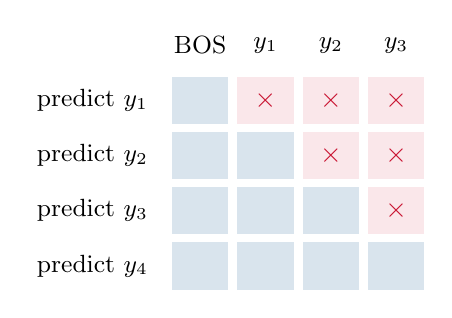
\begin{tikzpicture}[x=0.83cm,y=0.70cm]
        \foreach \c/\lab in {1/BOS,2/$y_1$,3/$y_2$,4/$y_3$}
          {\node[font=\small] at (\c,0) {\lab};}
        \foreach \r in {1,...,4} {
          \node[font=\small,anchor=east] at (0.35,-\r) {predict $y_\r$};
          \foreach \c in {1,...,4} {
            \ifnum\c>\r
              \fill[SlideRed!10] (\c-0.43,-\r-0.43) rectangle (\c+0.43,-\r+0.43);
              \node[text=SlideRed] at (\c,-\r) {$\times$};
            \else
              \fill[SlideBlue!15] (\c-0.43,-\r-0.43) rectangle (\c+0.43,-\r+0.43);
              \node[text=SlideBlue] at (\c,-\r) {$\checkmark$};
            \fi
          }
        }
      \end{tikzpicture}
      \par\smallskip{\small $\checkmark$ allowed\quad $\times$ blocked\quad BOS: start token}
    \end{column}
  \end{columns}
  \medskip
  \textbf{Training}: all target positions together.\quad
  \hot{Generation}: still one token at a time.
  \source{Vaswani et al., Sections 3.1 and 3.5. Mask grid: supplemental presenter illustration.}
\end{frame}

% Slide 8 | setup | 35 s. training.tex:6,10; results.tex:41,43.
\begin{frame}[label=setup]{Test translation quality and training cost}
  \takeaway{WMT 2014 translation; historical comparisons with reported training budgets.}
  \begin{columns}[t,onlytextwidth]
    \begin{column}{0.47\textwidth}
      \begin{block}{Data and evaluation}
        English--German: $\sim$4.5M sentence pairs.\par\smallskip
        English--French: 36M sentence pairs.\par\medskip
        Test set: \textbf{newstest2014}.\par
        BLEU $\uparrow$; beam size 4.\par
        Checkpoint averaging for test results.
      \end{block}
    \end{column}
    \begin{column}{0.47\textwidth}
      \begin{block}{One machine, 8 NVIDIA P100 GPUs}
        \textbf{Base}: 100K steps, about 12 hours.\par\medskip
        \textbf{Big}: 300K steps, about 3.5 days.\par\medskip
        Training FLOPs are estimates from time, GPU count, and GPU throughput.
      \end{block}
    \end{column}
  \end{columns}
  \bigskip
  \hot{Different systems used different budgets.}\par\smallskip
  Read Table 2 as a quality/cost comparison across published systems.
  \source{Vaswani et al., Sections 5.1--5.2 and 6.1. Main result discussion focuses on English--German.}
\end{frame}

% Slide 9 | results | 65 s. Original Table 2, PDF p. 8, rect [130,94,483,245].
% results.tex:16-26,37-43. Derived: 28.40 - 26.36 = 2.04 BLEU points.
% EN-FR discrepancy: Table 2 and abstract 41.8; Section 6.1 prose 41.0.
\begin{frame}[label=results]{28.4 BLEU on English--German}
  \takeaway{Transformer big exceeds the strongest prior EN--DE row by 2.04 BLEU points.}
  \begin{columns}[c,onlytextwidth]
    \begin{column}{0.76\textwidth}
      \includegraphics[width=\linewidth,height=4.7cm,keepaspectratio]{table2-original.pdf}
    \end{column}
    \begin{column}{0.21\textwidth}
      {\small EN--DE BLEU}\par\smallskip
      {\fontsize{28}{32}\selectfont\color{SlideBlue}\bfseries 28.4}\par
      {\small Transformer big}\par\medskip
      {\large 26.36}\par
      {\small ConvS2S ensemble}\par\medskip
      \good{+2.04 points}
    \end{column}
  \end{columns}
  \smallskip
  \textbf{Base}: 27.3 BLEU at an estimated $3.3\times10^{18}$ training FLOPs.
  \source{Original Table 2, Vaswani et al., v7; newstest2014. Bracketed IDs belong to the paper.\newline
    EN--FR discrepancy: Table 2 / abstract report 41.8; Section 6.1 prose reports 41.0.}
\end{frame}

% Slide 10 | ablation | 45 s. Original Table 3 headers/base/group A;
% PDF p. 9, rect [107,128,509,212]. results.tex:49,64-70,103-105.
% Derived: 25.8 - 24.9 = 0.9 BLEU; 8 and 16 heads tied at reported precision.
\begin{frame}[label=ablation]{More heads are not always better}
  \takeaway{On the development set, 8 and 16 heads tie; 32 heads score lower.}
  \centering
  \includegraphics[width=\textwidth,height=3.3cm,keepaspectratio]{table3-heads-original.pdf}
  \par\medskip
  \begin{columns}[t,onlytextwidth]
    \begin{column}{0.47\textwidth}
      \kw{One head $\rightarrow$ eight heads}\par\smallskip
      $24.9\rightarrow25.8$: \good{+0.9 BLEU points}.
    \end{column}
    \begin{column}{0.47\textwidth}
      \kw{Eight / sixteen / thirty-two heads}\par\smallskip
      $25.8\;/\;25.8\;/\;25.4$: a tie, then a decline.
    \end{column}
  \end{columns}
  \medskip
  \raggedright
  Head dimensions vary to keep computation comparable.\par\smallskip
  \textbf{newstest2013 (dev); no checkpoint averaging.}
  \source{Original Table 3, base row and group (A), Vaswani et al., v7.\newline
    Blank cells inherit the base settings. These scores are not the test scores on the previous page.}
\end{frame}

% Slide 11 | limits | 35 s. why_self_attention.tex:14-27,84-89; ms.tex:170-171.
% Scope caveat is presenter interpretation of layer-level asymptotics.
\begin{frame}[label=limits]{Shorter paths, quadratic attention cost}
  \takeaway{The efficiency advantage depends on sequence length and the operation being measured.}
  \begin{center}
    \renewcommand{\arraystretch}{1.5}
    \begin{tabular}{lccc}
      \toprule
      Layer type & Interaction cost & Sequential steps & Maximum path \\
      \midrule
      Self-attention & $O(n^2d)$ & $O(1)$ & $O(1)$ \\
      Recurrent & $O(nd^2)$ & $O(n)$ & $O(n)$ \\
      \bottomrule
    \end{tabular}
  \end{center}
  \smallskip
  $n$: sequence length; $d$: representation width.
  \begin{itemize}
    \item Full attention compares all pairs of positions.
    \item These are layer-level comparisons, not end-to-end latency guarantees.
    \item Autoregressive decoding retains a token-by-token dependency.
  \end{itemize}
  \source{Selected rows transcribed from Vaswani et al., Table 1; Sections 3.1, 4, and 7.\newline
    Full Transformer blocks also contain projections and feed-forward networks.}
\end{frame}

% Slide 12 | closing | 30 s. Synthesis of Sections 3,4,6; no new empirical claim.
\begin{frame}[label=closing]{Attention can carry sequence transduction}
  \takeaway{The contribution is a complete architecture, supported by translation evidence.}
  \vspace{0.25em}
  \begin{block}{1\quad Change how tokens communicate}
    Replace sequence-aligned recurrence with direct, learned attention.
  \end{block}
  \begin{block}{2\quad Make the architecture usable}
    Multi-head attention, positions, masking, feed-forward layers, and residual paths.
  \end{block}
  \begin{block}{3\quad Test quality and cost together}
    28.4 EN--DE BLEU; strong reported training efficiency, with explicit scope limits.
  \end{block}
  \vspace{0.3em}
  {\large\color{SlideBlue}\bfseries Thank you.}\hfill\textcolor{SlideGray}{Questions}
  \source{Vaswani et al., \emph{Attention Is All You Need}, NeurIPS 2017.}
\end{frame}

\appendix

% PDF page 13 | configuration | backup, 45 s. model_architecture.tex:18-20,119-124,146-155;
% training.tex:12-25,42. All numeric dimensions refer to base.
\begin{frame}[label=configuration]{Backup: the base model in precise terms}
  \takeaway{The 2017 architecture uses normalization after residual addition.}
  \begin{columns}[t,onlytextwidth]
    \begin{column}{0.46\textwidth}
      \kw{Dimensions}\par\smallskip
      $N=6$ per stack; $d_{\mathrm{model}}=512$.\par
      $h=8$; $d_k=d_v=64$; $d_{\mathrm{ff}}=2048$.
      \medskip\par
      \kw{Residual sublayer}\par\smallskip
      $\operatorname{LayerNorm}(x+\operatorname{Sublayer}(x))$\par
      Dropout on the sublayer output before addition.
      \medskip\par
      \kw{Position-wise feed-forward network}\par\smallskip
      $\max(0,xW_1+b_1)W_2+b_2$
    \end{column}
    \begin{column}{0.49\textwidth}
      \kw{Sinusoidal position encoding}
      \begin{align*}
        PE_{(p,2i)} &= \sin(p/10000^{2i/d_{\mathrm{model}}}) \\
        PE_{(p,2i+1)} &= \cos(p/10000^{2i/d_{\mathrm{model}}})
      \end{align*}
      $p$: token position; $i$: dimension-pair index.
      \medskip\par
      \kw{Training}\par\smallskip
      Adam; 4,000-step learning-rate warmup.\par
      Base dropout: 0.1; label smoothing: 0.1.
    \end{column}
  \end{columns}
  \source{Vaswani et al., Sections 3.1, 3.3, 3.5, 5.3, and 5.4.}
\end{frame}

% PDF page 14 | score-notes | backup, 45 s. results.tex:26,39,41,64,91,103.
% Original prose excerpt PDF p. 8 [107,488,505,531]; local discrepancy preserved.
\begin{frame}[label=score-notes]{Backup: keep the score conditions attached}
  \takeaway{The v7 English--French discrepancy remains unresolved in the paper.}
  \kw{Transformer big, English--French}\par\smallskip
  Table 2 and abstract: \textbf{41.8 BLEU}.\quad Section 6.1 prose: \hot{41.0 BLEU}.
  \begin{center}
    \includegraphics[width=0.94\textwidth,height=1.65cm,keepaspectratio]{enfr-prose-original.pdf}
  \end{center}
  \begin{columns}[t,onlytextwidth]
    \begin{column}{0.47\textwidth}
      \kw{Test $\ne$ development}\par\smallskip
      Table 2: newstest2014, checkpoint averaging.\par
      Table 3: newstest2013, no checkpoint averaging.
    \end{column}
    \begin{column}{0.47\textwidth}
      \kw{Positional encoding ablation}\par\smallskip
      Sinusoidal: 25.8 dev BLEU.\par
      Learned: 25.7 dev BLEU.\par
      Close reported scores; no significance claim.
    \end{column}
  \end{columns}
  \source{Original prose excerpt: Vaswani et al., v7, Section 6.1, PDF p. 8.\newline
    Table 3 base / row (E); Section 6.2. No silent correction or averaging of the conflicting values.}
\end{frame}

% PDF page 15 | references | backup, 20 s. Local BibTeX database.
\begin{frame}[label=references]{Backup: reference and source version}
  \takeaway{All original figures and table excerpts come from the same paper version.}
  \nocite{vaswani2017attention}
  \bibliographystyle{plain}
  \bibliography{strings,refs}
  \bigskip
  \small
  \url{https://arxiv.org/abs/1706.03762v7}\par\medskip
  Figures 1--2: original standalone PNG assets.\par
  Figure 1 detail and table excerpts: crops from the matching PDF.\par\medskip
  The paper grants attributed figure/table reproduction for journalistic or scholarly works.
  \source{Retrieved 26 September 2026. Detailed provenance and transformations: sources.md.}
\end{frame}
\end{document}
